\documentclass{beamer}

% xcolor and define colors -------------------------
\usepackage{xcolor}

% https://www.viget.com/articles/color-contrast/
\definecolor{purple}{HTML}{5601A4}
\definecolor{navy}{HTML}{0D3D56}
\definecolor{ruby}{HTML}{9a2515}
\definecolor{alice}{HTML}{107895}
\definecolor{daisy}{HTML}{EBC944}
\definecolor{coral}{HTML}{F26D21}
\definecolor{kelly}{HTML}{829356}
\definecolor{cranberry}{HTML}{E64173}
\definecolor{jet}{HTML}{131516}
\definecolor{asher}{HTML}{555F61}
\definecolor{slate}{HTML}{314F4F}

% Mixtape Sessions
\definecolor{picton-blue}{HTML}{00b7ff}
\definecolor{violet-red}{HTML}{ff3881}
\definecolor{sun}{HTML}{ffaf18}
\definecolor{electric-violet}{HTML}{871EFF}

\newcommand\pictonBlue[1]{{\color{picton-blue}#1}}
\newcommand\sun[1]{{\color{sun}#1}}
\newcommand\electricViolet[1]{{\color{electric-violet}#1}}
\newcommand\violetRed[1]{{\color{violet-red}#1}}

\newcommand\bgPictonBlue[1]{{\colorbox{picton-blue!20!white}{#1}}}
\newcommand\bgSun[1]{{\colorbox{sun!20!white}{#1}}}
\newcommand\bgElectricViolet[1]{{\colorbox{electric-violet!20!white}{#1}}}
\newcommand\bgVioletRed[1]{{\colorbox{violet-red!20!white}{#1}}}

\def\code#1{\texttt{#1}}

% Main theme colors
\definecolor{accent}{HTML}{00b7ff}
\definecolor{accent2}{HTML}{871EFF}
\definecolor{gray100}{HTML}{f3f4f6}
\definecolor{gray800}{HTML}{1F292D}


% Beamer Options -------------------------------------

% Background
\setbeamercolor{background canvas}{bg = white}

% Change text margins
\setbeamersize{text margin left = 15pt, text margin right = 15pt} 

% \alert
\setbeamercolor{alerted text}{fg = accent2}

% Frame title
\setbeamercolor{frametitle}{bg = white, fg = jet}
\setbeamercolor{framesubtitle}{bg = white, fg = accent}
\setbeamerfont{framesubtitle}{size = \small, shape = \itshape}

% Block
\setbeamercolor{block title}{fg = white, bg = accent2}
\setbeamercolor{block body}{fg = gray800, bg = gray100}

% Title page
\setbeamercolor{title}{fg = gray800}
\setbeamercolor{subtitle}{fg = accent}

%% Custom \maketitle and \titlepage
\setbeamertemplate{title page}
{
    %\begin{centering}
        \vspace{20mm}
        {\Large \usebeamerfont{title}\usebeamercolor[fg]{title}\inserttitle}\\
        {\large \itshape \usebeamerfont{subtitle}\usebeamercolor[fg]{subtitle}\insertsubtitle}\\ \vspace{10mm}
        {\insertauthor}\\
        {\color{asher}\small{\insertdate}}\\
    %\end{centering}
}

% Table of Contents
\setbeamercolor{section in toc}{fg = accent!70!jet}
\setbeamercolor{subsection in toc}{fg = jet}

% Button 
\setbeamercolor{button}{bg = accent}

% Remove navigation symbols
\setbeamertemplate{navigation symbols}{}

% Table and Figure captions
\setbeamercolor{caption}{fg=jet!70!white}
\setbeamercolor{caption name}{fg=jet}
\setbeamerfont{caption name}{shape = \itshape}

% Bullet points

%% Fix spacing between items
\let\olditemize=\itemize 
\let\endolditemize=\enditemize 
\renewenvironment{itemize}{\vspace{0.25em}\olditemize \itemsep0.25em}{\endolditemize}

%% Fix left-margins
\settowidth{\leftmargini}{\usebeamertemplate{itemize item}}
\addtolength{\leftmargini}{\labelsep}

%% enumerate item color
\setbeamercolor{enumerate item}{fg = accent}
\setbeamerfont{enumerate item}{size = \small}
\setbeamertemplate{enumerate item}{\insertenumlabel.}

%% itemize
\setbeamercolor{itemize item}{fg = accent!70!white}
\setbeamerfont{itemize item}{size = \small}
\setbeamertemplate{itemize item}[circle]

%% right arrow for subitems
\setbeamercolor{itemize subitem}{fg = accent!60!white}
\setbeamerfont{itemize subitem}{size = \small}
\setbeamertemplate{itemize subitem}{$\rightarrow$}

\setbeamertemplate{itemize subsubitem}[square]
\setbeamercolor{itemize subsubitem}{fg = jet}
\setbeamerfont{itemize subsubitem}{size = \small}








% Links ----------------------------------------------

\usepackage{hyperref}
\hypersetup{
  colorlinks = true,
  linkcolor = accent2,
  filecolor = accent2,
  urlcolor = accent2,
  citecolor = accent2,
}


% Line spacing --------------------------------------
\usepackage{setspace}
\setstretch{1.35}


% \begin{columns} -----------------------------------
\usepackage{multicol}


% Fonts ---------------------------------------------
% Beamer Option to use custom fonts
\usefonttheme{professionalfonts}

% \usepackage[utopia, smallerops, varg]{newtxmath}
% \usepackage{utopia}
\usepackage[sfdefault,light]{roboto}

% Small adjustments to text kerning
\usepackage{microtype}



% Remove annoying over-full box warnings -----------
\vfuzz2pt 
\hfuzz2pt


% Table of Contents with Sections
\setbeamerfont{myTOC}{series=\bfseries, size=\Large}
\AtBeginSection[]{
        \frame{
            \frametitle{Roadmap}
            \tableofcontents[current]   
        }
    }


% Tables -------------------------------------------
% Tables too big
% \begin{adjustbox}{width = 1.2\textwidth, center}
\usepackage{adjustbox}
\usepackage{array}
\usepackage{threeparttable, booktabs, adjustbox}
    
% Fix \input with tables
% \input fails when \\ is at end of external .tex file
\makeatletter
\let\input\@@input
\makeatother

% Tables too narrow
% \begin{tabularx}{\linewidth}{cols}
% col-types: X - center, L - left, R -right
% Relative scale: >{\hsize=.8\hsize}X/L/R
\usepackage{tabularx}
\newcolumntype{L}{>{\raggedright\arraybackslash}X}
\newcolumntype{R}{>{\raggedleft\arraybackslash}X}
\newcolumntype{C}{>{\centering\arraybackslash}X}

% Figures

% \imageframe{img_name} -----------------------------
% from https://github.com/mattjetwell/cousteau
\newcommand{\imageframe}[1]{%
    \begin{frame}[plain]
        \begin{tikzpicture}[remember picture, overlay]
            \node[at = (current page.center), xshift = 0cm] (cover) {%
                \includegraphics[keepaspectratio, width=\paperwidth, height=\paperheight]{#1}
            };
        \end{tikzpicture}
    \end{frame}%
}

% subfigures
\usepackage{subfigure}


% Highlight slide -----------------------------------
% \begin{transitionframe} Text \end{transitionframe}
% from paulgp's beamer tips
\newenvironment{transitionframe}{
    \setbeamercolor{background canvas}{bg=accent!40!black}
    \begin{frame}\color{accent!10!white}\LARGE\centering
}{
    \end{frame}
}


% Table Highlighting --------------------------------
% Create top-left and bottom-right markets in tabular cells with a unique matching id and these commands will outline those cells
\usepackage[beamer,customcolors]{hf-tikz}
\usetikzlibrary{calc}
\usetikzlibrary{fit,shapes.misc}

% To set the hypothesis highlighting boxes red.
\newcommand\marktopleft[1]{%
    \tikz[overlay,remember picture] 
        \node (marker-#1-a) at (0,1.5ex) {};%
}
\newcommand\markbottomright[1]{%
    \tikz[overlay,remember picture] 
        \node (marker-#1-b) at (0,0) {};%
    \tikz[accent!80!jet, ultra thick, overlay, remember picture, inner sep=4pt]
        \node[draw, rectangle, fit=(marker-#1-a.center) (marker-#1-b.center)] {};%
}


% DAGS ----------------------------------------------
\usepackage{tikz}
\usetikzlibrary{shapes,decorations,arrows,calc,arrows.meta,fit,positioning}
% Tikz settings optimized for causal graphs.
\tikzset{
    -Latex,auto,node distance =1 cm and 1 cm,semithick,
    state/.style ={ellipse, draw, minimum width = 0.7 cm},
    point/.style = {circle, draw, inner sep=0.04cm,fill,node contents={}},
    bidirected/.style={Latex-Latex,dashed},
    el/.style = {inner sep=2pt, align=left, sloped}
}


% Beamer tricks -------------------------------------
% Make \pause work in align environments
\makeatletter
\renewrobustcmd{\beamer@@pause}[1][]{%
  \unless\ifmeasuring@%
  \ifblank{#1}%
    {\stepcounter{beamerpauses}}%
    {\setcounter{beamerpauses}{#1}}%
  \onslide<\value{beamerpauses}->\relax%
  \fi%
}
\makeatother

\usepackage{breqn} % Breaks lines

\usepackage{amsmath}
\usepackage{mathtools}

\usepackage{pdfpages} % \includepdf

\usepackage{listings} % R code
\usepackage{verbatim} % verbatim

% Video stuff
\usepackage{media9}

% packages for bibs and cites
\usepackage{natbib}
\usepackage{har2nat}
\newcommand{\possessivecite}[1]{\citeauthor{#1}'s \citeyearpar{#1}}
\usepackage{breakcites}
\usepackage{alltt}

% Setup math operators
\DeclareMathOperator{\E}{E} \DeclareMathOperator{\tr}{tr} \DeclareMathOperator{\se}{se} \DeclareMathOperator{\I}{I} \DeclareMathOperator{\sign}{sign} \DeclareMathOperator{\supp}{supp} \DeclareMathOperator{\plim}{plim}
\DeclareMathOperator*{\dlim}{\mathnormal{d}\mkern2mu-lim}
\newcommand\independent{\protect\mathpalette{\protect\independenT}{\perp}}
   \def\independenT#1#2{\mathrel{\rlap{$#1#2$}\mkern2mu{#1#2}}}
\newcommand*\colvec[1]{\begin{pmatrix}#1\end{pmatrix}}

\newcommand{\myurlshort}[2]{\href{#1}{\textcolor{gray}{\textsf{#2}}}}


\begin{document}

\imageframe{./lecture_includes/mixtape_did_cover.png}


% ---- Content ----

   
\section{Synthetic control}

\subsection{Abadie, Diamond and Hainmueller}


\begin{frame}[plain]
	\begin{figure}
	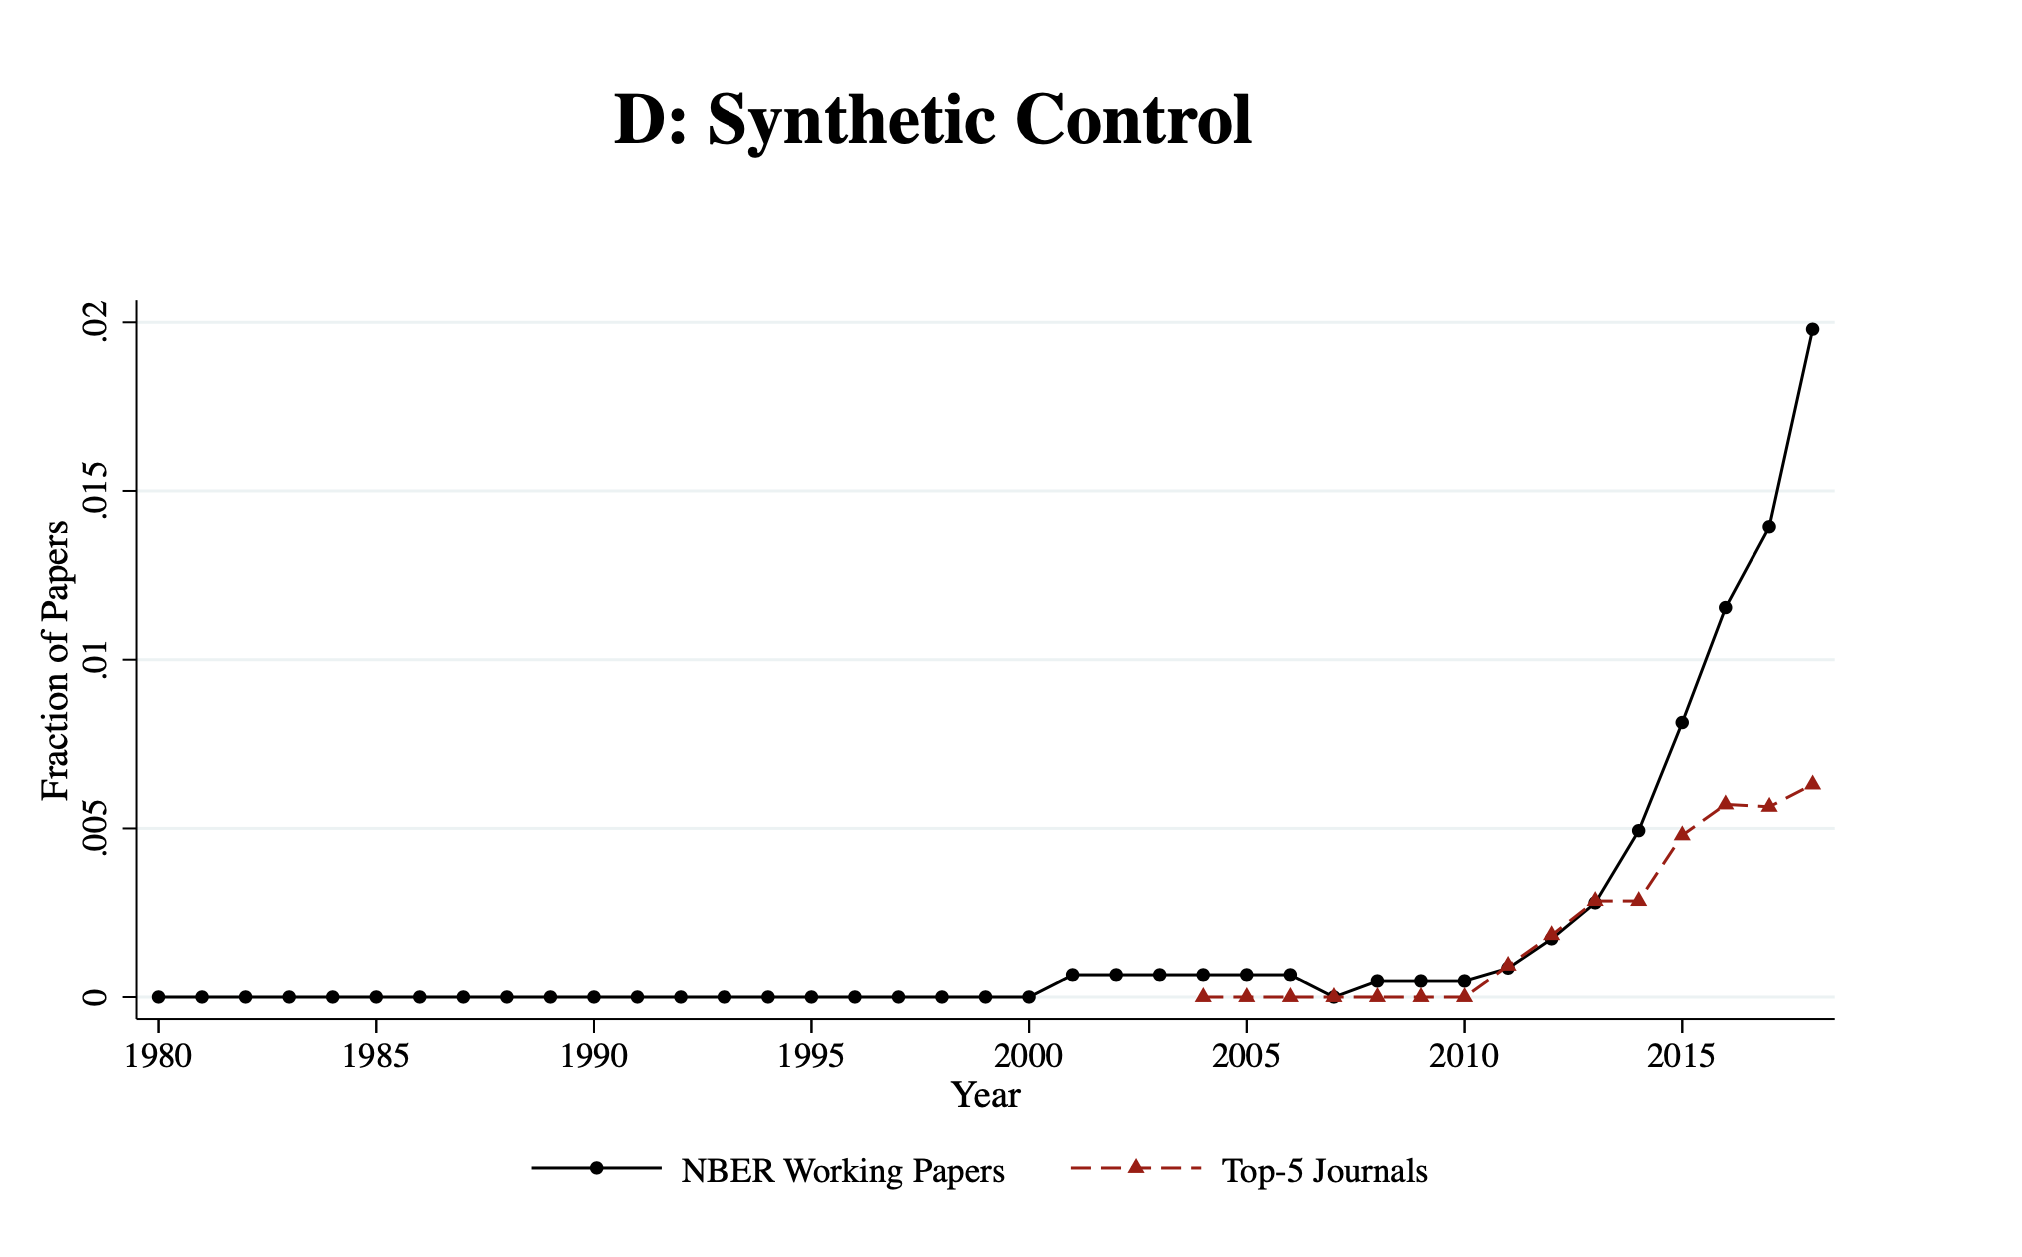
\includegraphics[scale=0.25]{./lecture_includes/currie_synth.png}
	\end{figure}
\end{frame}

\begin{frame}{What is synthetic control}
	
	\begin{itemize}
	\item Synthetic control has been called the most important innovation in causal inference of the last two decades (Athey and Imbens 2017)
	\item Originally designed for comparative case studies, but newer developments have extended it to multiple treated units as well as differential timing
	\item Continues to also be methodologically a frontier for applied econometrics, so consider this talk a starting point for you
	\end{itemize}
\end{frame}
	
\begin{frame}{What is a comparative case study}

\begin{itemize}
\item Comparative case studies compare a single unit to another unit to make causal inference
\item Single treated unit is usually a country, state, firm, etc.
\item Social scientists traditionally tackled them either qualitatively and quantitatively (more traditional economic approach)
\end{itemize}

\end{frame}


\begin{frame}{Qualitative comparative case studies}
	
	\begin{itemize}
	\item In qualitative comparative case studies, the goal might be to reason \emph{inductively} the causal effects of events or characteristics of a single unit on some outcome, oftentimes through logic and historical analysis.  
		\begin{itemize}
		\item Classic example of comparative case study approach is Alexis de Toqueville's \underline{Democracy in America} (but he is regularly comparing the US to France)
		\end{itemize}
	\item Sometimes there may not be an explicit counterfactual, or if there is, it's not principled (subjective researcher decision)
	\item Quantitative claims about causal effects are unlikely -- de Toqueville's won't claim GDP per capita fell \$500 when compared against France
	\end{itemize}
\end{frame}

\begin{frame}{Traditional quantitative comparative case studies}

\begin{itemize}
	\item Traditional quantitative comparative case studies are explicitly causal designs in that there is a treatment and control, usually involving natural experiment on a single aggregate unit
	\item Comparison focuses on the the evolution of an aggregate outcome for the unit affected by the intervention to the evolution of the same \emph{ad hoc} aggregate control group (Card 1990; Card and Krueger 1994)
	\item It'll essentially be diff-in-diff, but it may not use the event study, and the point is the choice of controls is a subset of all possible controls
\end{itemize}

\end{frame}

\begin{frame}{Pros and cons}
	
	\begin{itemize}
	\item Pros:
		\begin{itemize}
		\item Takes advantage of policy interventions that take place at an aggregate level (which is common and so this is useful)
		\item Aggregate/macro data are often available (which may be all we have)
		\end{itemize}
	\item Cons:
		\begin{itemize}
		\item Selection of control group is \emph{ad hoc} -- opens up researcher biases, even unconscious
		\item Standard errors do not reflect uncertainty about the ability of the control group to reproduce the counterfactual of interest
		\end{itemize}
	\end{itemize}
\end{frame}

\begin{frame}{Description of the Mariel Boatlift}
	
	\begin{itemize}
	\item In 1980, Fidel Castro allowed anyone to leave Cuba so long as they did in the fall from the Mariel boat dock.
	\item The Mariel Boatlift brought 100,000 Cubans to Miami which increased the Miami labor force by 7\%
	\item Card (1990) uses the Mariel Boatlift as a natural experiment to measure the effect of a sudden influx of immigrants on unemployment among less-skilled natives
	\item His question was how do inflows of immigrants affect the wages and employment of natives in local US labor markets?
	\item Individual-level data on unemployment from the Current Population Survey (CPS) for Miami and comparison cities
	\end{itemize}
\end{frame}


\begin{frame}[plain]
	\begin{figure}
	
\includegraphics[scale=0.25]{./lecture_includes/boatlift2.png}
	\end{figure}
\end{frame}

\begin{frame}[plain]
	\begin{figure}
	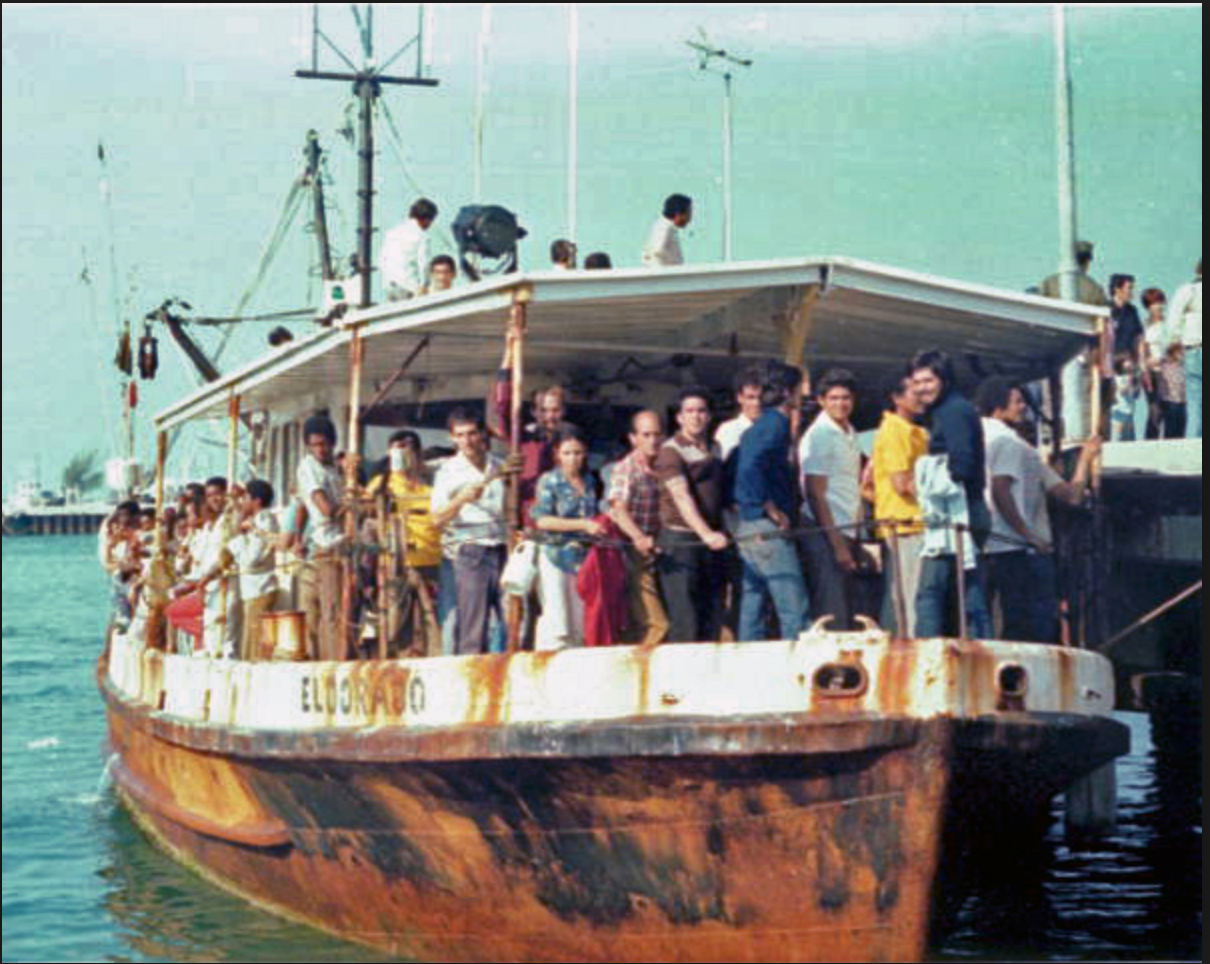
\includegraphics[scale=0.25]{./lecture_includes/boatlift3.png}
	\end{figure}
\end{frame}

\begin{frame}[plain]
	\begin{figure}
	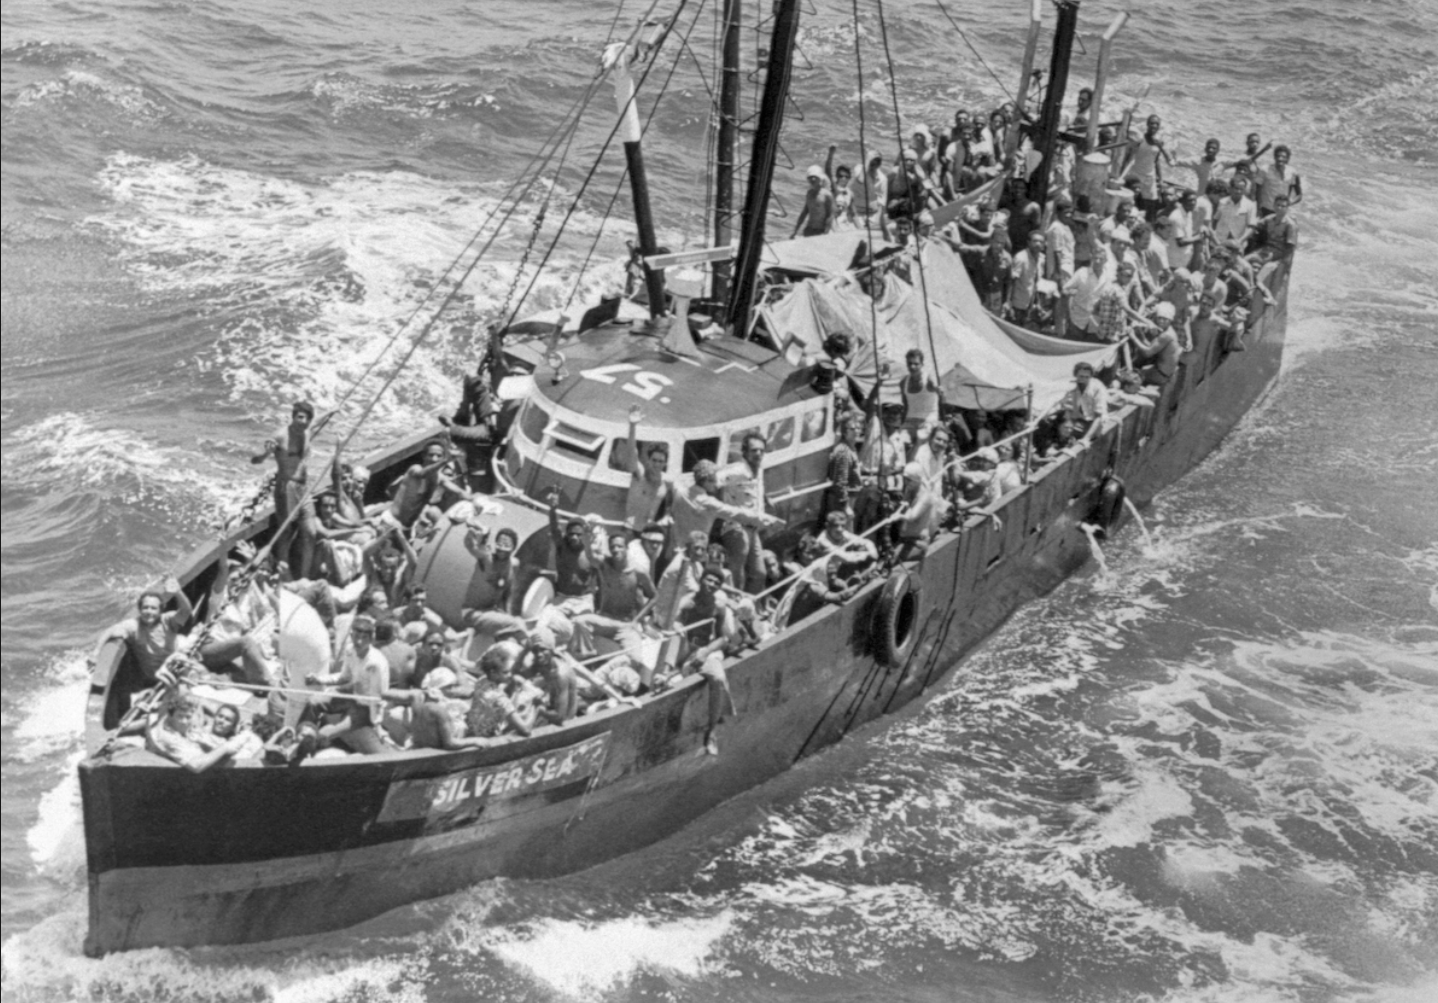
\includegraphics[scale=0.25]{./lecture_includes/boatlift4.png}
	\end{figure}
\end{frame}


\begin{frame}{Selecting control groups}

\begin{itemize}

\item His treatment group was low skill workers in Miami since that's where Cubans went
\item But which control group?
\item He chose Atlanta, Los Angeles, Houston, Tampa-St. Petersburg

\end{itemize}

\end{frame}



\begin{frame}{Why these four?}

	\begin{figure}
	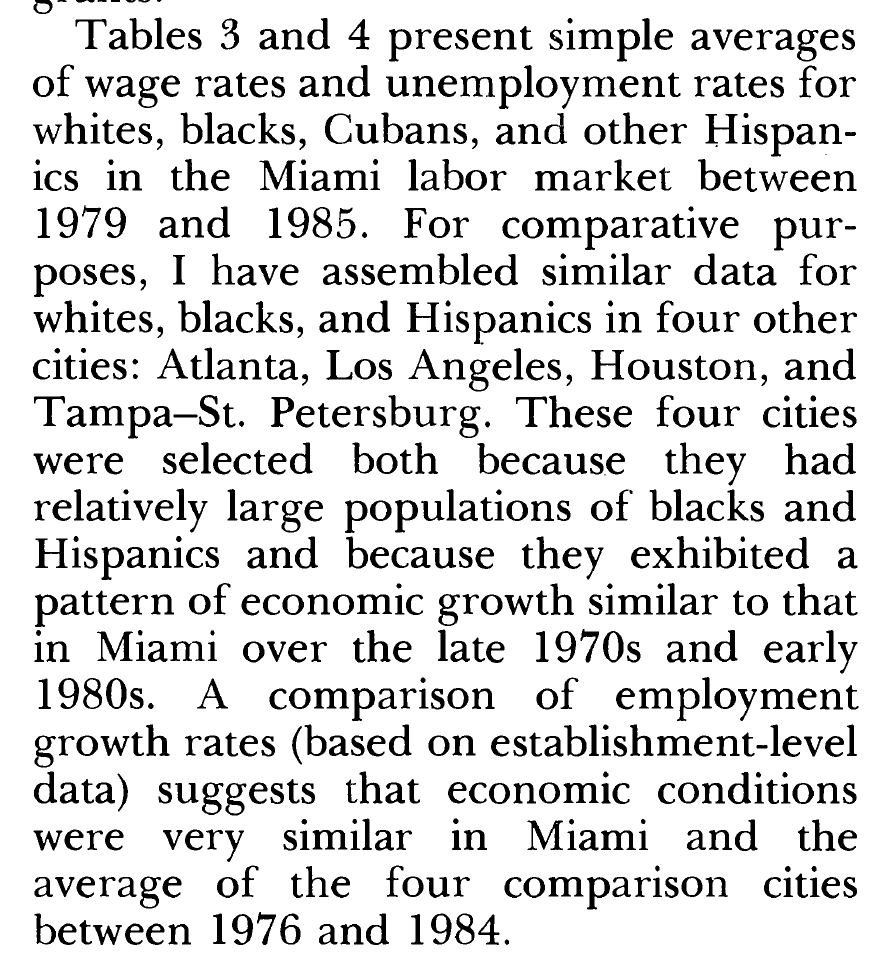
\includegraphics[scale=0.25]{./lecture_includes/card_illr.png}
	\end{figure}

\end{frame}

\begin{frame}{Diff-in-diff}
	
	\begin{figure}
	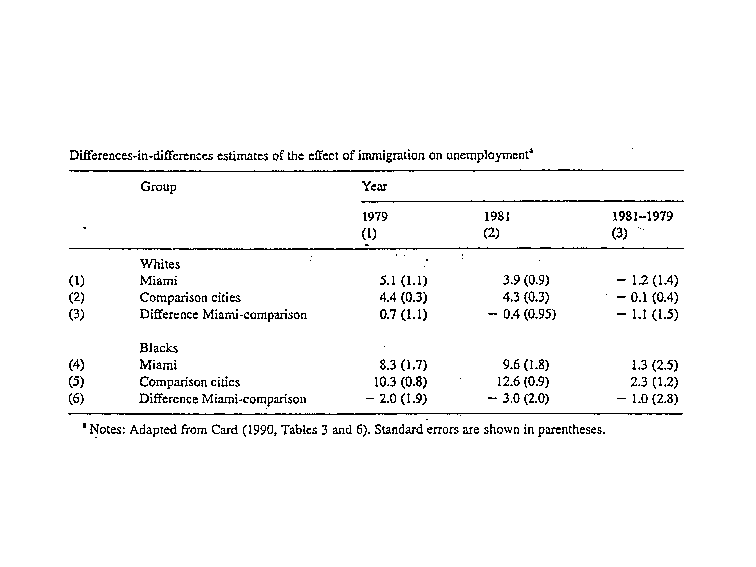
\includegraphics[scale=0.75]{./lecture_includes/abadie_2.pdf}
	\end{figure}
\end{frame}

\begin{frame}{Parallel trends}

\begin{itemize}
\item His estimate is unbiased if the change in $Y^0$ for the comparison cities correctly approximates the unobserved $\textcolor{red}{\Delta Y^0}$ for the treatment group
\item But Card largely focused on covariates, and in a relatively casual way (``similar growth'') and does not report much
\item Black result would have been positive, too, were it not that the comparison cities growth was smaller -- uncertainty about null result being from no effect or arbitrary control group
\end{itemize}

\end{frame}


\begin{frame}{Synthetic Control}
	
	\begin{itemize}
	\item Abadie and Gardeazabal (2003) introduced synthetic control in the AER in a study of a terrorist attack in Spain (Basque) on GDP
	\item Revisited again in a 2010 JASA with Diamond and Hainmueller, two political scientists who were PhD students at Harvard (more proofs and inference)
	\item Basic idea is to use a combination of comparison units as counterfactual for a treated unit where the units are chosen according to a data driven procedure
	\end{itemize}
\end{frame}


\begin{frame}{Researcher's objectives}

\begin{itemize}
	\item Our goal here is to reproduce the counterfactual of a treated unit by finding the combination of untreated units that best resembles the treated unit \emph{before} the intervention in terms of the values of $k$ relevant covariates (predictors of the outcome of interest)
	\item Method selects \emph{weighted average of all potential comparison units} that best resembles the characteristics of the treated unit(s) - called the ``synthetic control''
\end{itemize}

\end{frame}

\begin{frame}{Synthetic control method: advantages}
	
	\begin{itemize}
	\item ``Convex hull'' means synth is a weighted average of units which means the counterfactual is a collection of comparison units that on average track the treatment group over time.
	\item Constraints on the model use non-negative weights which does not allow for extrapolation 
	\item Makes explicit the contribution of each comparison unit to the counterfactual 
	\item Formalizing the way comparison units are chosen has direct implications for inference
	\end{itemize}
\end{frame}


\begin{frame}{Synthetic control method: disadvantages}

\begin{enumerate}
\item Subjective researcher bias kicked down to the model selection stage
\item Significant diversity at the moment as to how to principally select models - from machine learning to modifications - as well as estimation and software
\item Part of the purpose of this procedure is to reduce subjective researcher bias
\item Ferman, Pinto and Possbaum (2020) suggest specific specifications and report all of them
\end{enumerate}

\end{frame}


\begin{frame}{Avoiding cherry picking}

	\begin{figure}
	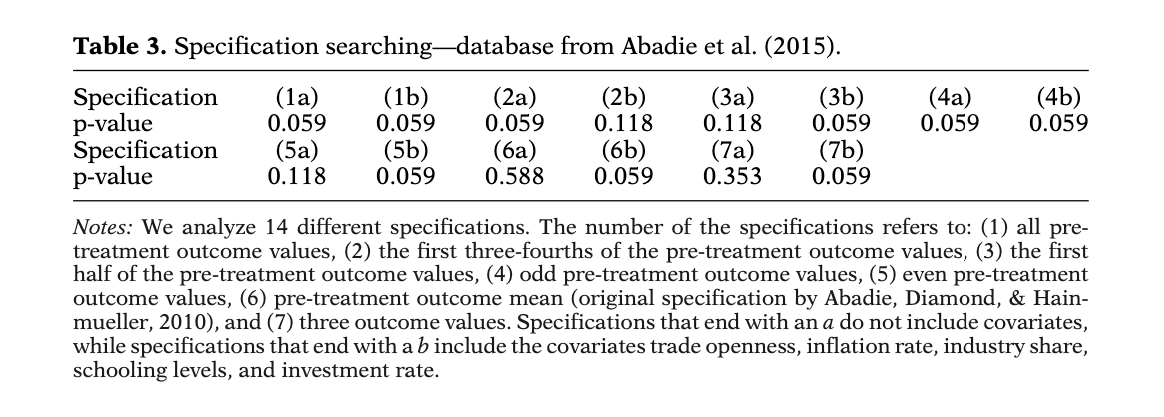
\includegraphics[scale=0.5]{./lecture_includes/cherry_picking_1.png}
	\end{figure}

\end{frame}

\begin{frame}{Avoiding cherry picking}

	\begin{figure}
	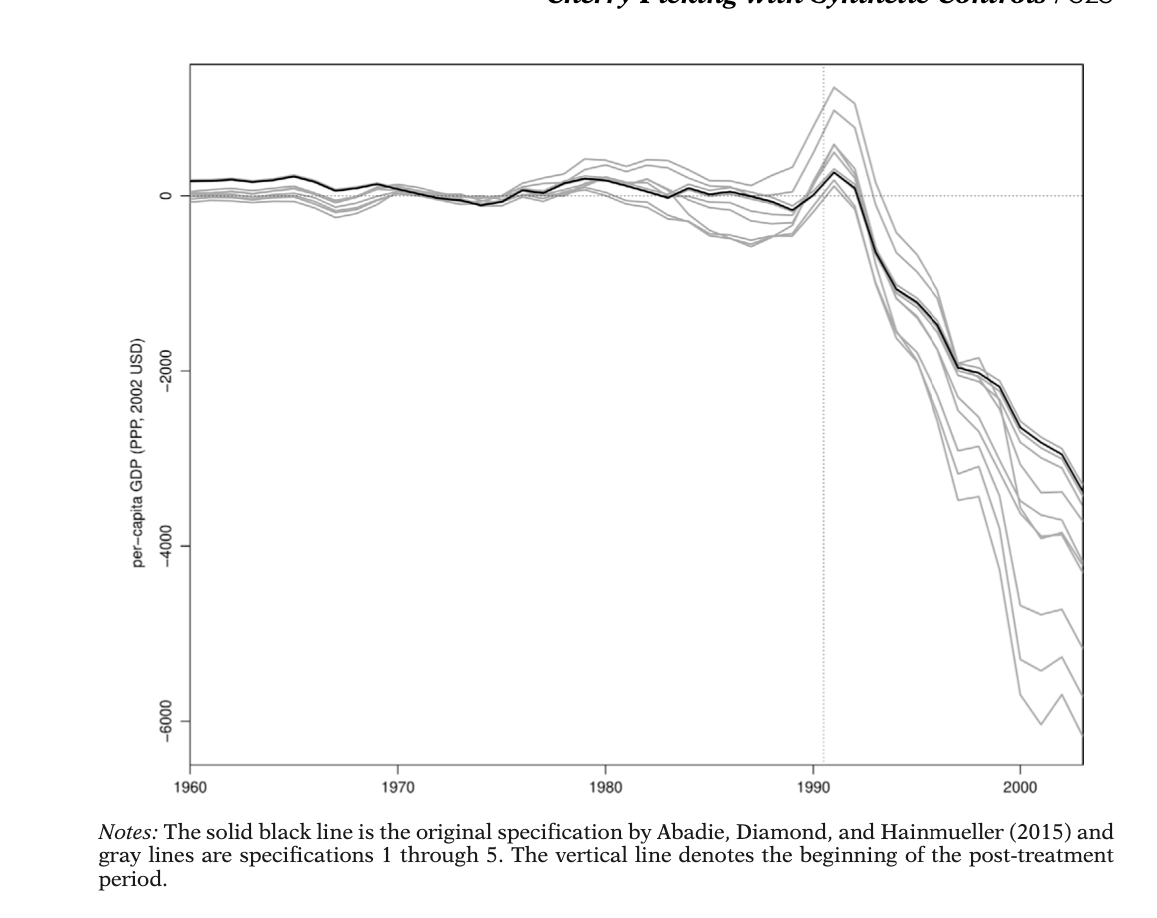
\includegraphics[scale=0.5]{./lecture_includes/cherry_picking_2.png}
	\end{figure}

\end{frame}


\begin{frame}{Notation and setup}
	
Suppose that we observe $J+1$ units in periods $1, 2, \dots, T$
		\begin{itemize}
		\item Unit ``one'' is exposed to the intervention of interest (that is, ``treated'') during periods $T_0+1, \dots, T$
		\item The remaining $J$ are an untreated reservoir of potential controls (a ``donor pool'')
		\end{itemize}	
\end{frame}


\begin{frame}{Potential outcomes notation}

		\begin{itemize}
		\item Let $Y_{it}^0$ be the outcome that would be observed for unit $i$ at time $t$ in the absence of the intervention
		\item Let $Y_{it}^1$ be the outcome that would be observed for unit $i$ at time $t$ if unit $i$ is exposed to the intervention in periods $T_0+1$ to $T$.
		\end{itemize}

\end{frame}

\begin{frame}{Group-time ATT with only one treated group}

Treatment effect parameter is defined as dynamic ATT where 

\begin{eqnarray*}
\delta_{1t}&=&Y_{1t}^1 - Y_{1t}^0 \\
&=& Y_{1t} - Y_{1t}^0 
\end{eqnarray*} for each post-treatment period, $t>T_0$ and $Y_{1t}$ is the outcome for unit one at time $t$. We will estimate $Y^0_{1t}$ using the $J$ units in the donor pool 

\end{frame}

\begin{frame}{Optimal weights}
	
	\begin{itemize}
	\item Let $W=(w_2, \dots, w_{J+1})'$ with $w_j\geq 0$ for $j=2, \dots, J+1$ and $w_2+\dots+w_{j+1}=1$. Each value of $W$ represents a potential synthetic control
	\item Let $X_1$ be a $(k\times 1)$ vector of pre-intervention characteristics for the treated unit.  Similarly, let $X_0$ be a $(k\times J)$ matrix which contains the same variables for the unaffected units.
	\item The vector $W^*=(w_2^*, \dots, w_{J+1}^*)'$ is chosen to minimize $||X_1-X_0W||$, subject to our weight constraints
	\end{itemize}
\end{frame}

\begin{frame}{Optimal weights differ by another weighting matrix}
	
Abadie, et al. consider $$||X_1 - X_0W||=\sqrt{(X_1-X_0W)'V(X_1-X_0W)}$$where $X_{jm}$ is the value of the $m$-th covariates for unit $j$ and $V$ is some $(k\times k)$ symmetric and positive semidefinite matrix

\end{frame}

\begin{frame}{More on the V matrix}

Typically, $V$ is diagonal with main diagonal $v_1, \dots, v_k$.  Then, the synthetic control weights $w_2^*, \dots, w_{J+1}^*$ minimize: $$\sum_{m=1}^k v_m \bigg(X_{1m} - \sum_{j=2}^{J+1}w_jX_{jm}\bigg)^2$$ where $v_m$ is a weight that reflects the relative importance that we assign to the $m$-th variable when we measure the discrepancy between the treated unit and the synthetic controls

\end{frame}

\begin{frame}{Choice of $V$ is critical}
	
		\begin{itemize}
		\item The synthetic control $W^*(V^*)$ is meant to reproduce the behavior of the outcome variable for the treated unit in the absence of the treatment
		\item Therefore, the $V^*$ weights directly shape $W^*$
		\end{itemize}
\end{frame}

\begin{frame}{Estimating the $V$ matrix}
	
 Choice of $v_1, \dots, v_k$ can be based on
		\begin{itemize}
		\item Assess the predictive power of the covariates using regression
		\item Subjectively assess the predictive power of each of the covariates, or calibration inspecting how different values for $v_1, \dots, v_k$ affect the discrepancies between the treated unit and the synthetic control
		\item Minimize mean square prediction error (MSPE) for the pre-treatment period (default):
			\begin{eqnarray*}
			\sum_{t=1}^{T_0} \bigg(Y_{1t} - \sum_{j=2}^J w_j^*(V^*)Y_{jt} \bigg)^2
			\end{eqnarray*}
		\end{itemize}
\end{frame}

\begin{frame}{Cross validation}

\begin{itemize}
		\item Divide the pre-treatment period into an initial \textbf{training} period and a subsequent \textbf{validation} period
		\item For any given $V$, calculate $W^*(V)$ in the training period.
		\item Minimize the MSPE of $W^*(V)$ in the validation period
\end{itemize}

\end{frame}


\begin{frame}{Suppose $Y^0$ is given by a factor model}

Synthetic control does not use the parallel trends assumption; it uses a factor model assumption 

\bigskip

Assume potential outcome, $Y^0$ follows dynamic path based on observed and unobserved heterogeneity:
\begin{eqnarray*}
Y_{it}^0 = \alpha_t + \theta_t Z_i + \lambda_t u_i + \varepsilon_{it}
\end{eqnarray*}where $\alpha_t$ is an unknown common factor with constant factor loadings across units, and $\lambda_t$ is a vector of unobserved common factors

\bigskip

Synthetic control will also follow that path

\end{frame}

\begin{frame}{With some manipulation}

\begin{eqnarray*}
Y^0_{1t} - \sum^{J+1}_{j=2}w^*_jY_{jt} &=& \sum_{j=2}^{J+1} w_j^* \sum_{s=1}^{T_0} \lambda_t \bigg ( \sum_{n=1}^{T_0} \lambda_n'\lambda_n \bigg )
^{-1} \lambda_s'(\varepsilon_{js} - \varepsilon_{1s} ) \\
&& - \sum_{j=2}^{J+1} w_j^* (\varepsilon_{jt} - \varepsilon_{1t})
\end{eqnarray*}

\begin{itemize}
\item If $\sum_{t=1}^{T_0} \lambda_t' \lambda_t$ is nonsingular, then RHS will be close to zero if number of preintervention periods is ``large''  relative to size of transitory shocks 
\item Only units that are alike in observables and unobservables should produce similar trajectories of the outcome variable over extended periods of time
\item Proof in Appendix B of ADH (2011)
\end{itemize}


\end{frame}


\begin{frame}{Example: California's Proposition 99}
	
	\begin{itemize}
	\item In 1988, California first passed comprehensive tobacco control legislation:
		\begin{itemize}
		\item increased cigarette tax by 25 cents/pack
		\item earmarked tax revenues to health and anti-smoking budgets
		\item funded anti-smoking media campaigns
		\item spurred clean-air ordinances throughout the state
		\item produced more than \$100 million per year in anti-tobacco projects
		\end{itemize}
	\item Other states that subsequently passed control programs are excluded from donor pool of controls (AK, AZ, FL, HI, MA, MD, MI, NJ, OR, WA, DC)
	\end{itemize}
\end{frame}

\begin{frame}{Cigarette Consumption: CA and the Rest of the US}
	
	\begin{figure}
	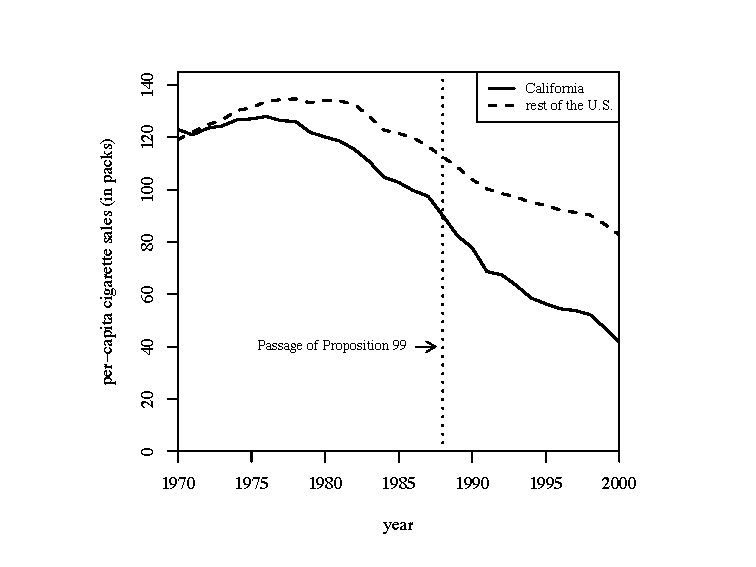
\includegraphics[scale=0.75]{./lecture_includes/abadie_3.pdf}
	\end{figure}
\end{frame}

\begin{frame}{Cigarette Consumption: CA and synthetic CA}
	
	\begin{figure}
	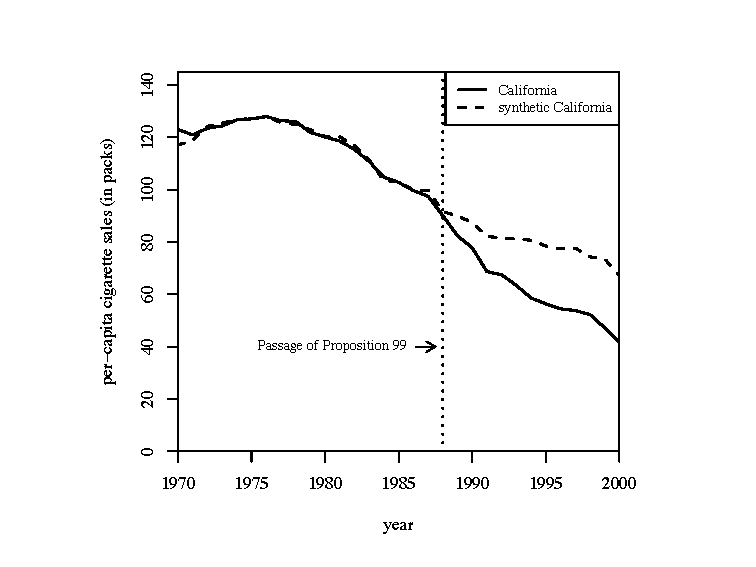
\includegraphics[scale=0.75]{./lecture_includes/abadie_4.pdf}
	\end{figure}
\end{frame}

\begin{frame}{Predictor Means: Actual vs. Synthetic California}
	
	\begin{figure}
	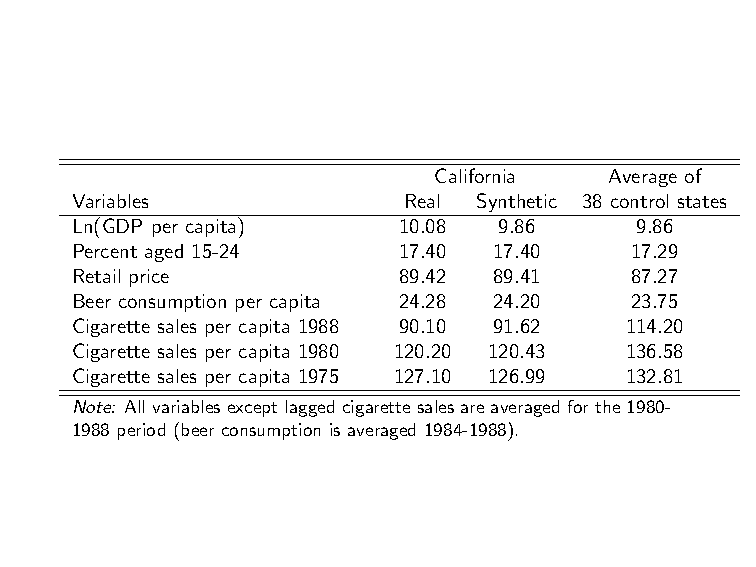
\includegraphics[scale=0.75]{./lecture_includes/abadie_5.pdf}
	\end{figure}
\end{frame}

\begin{frame}{Smoking Gap between CA and synthetic CA}
	
	\begin{figure}
	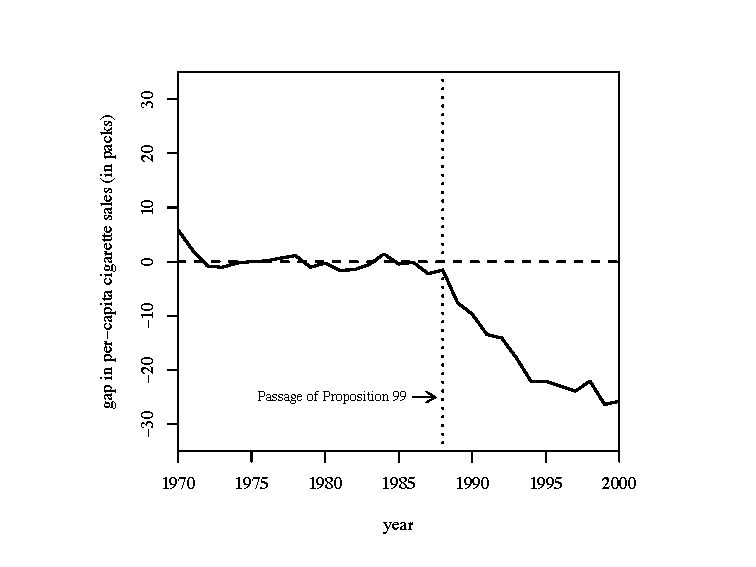
\includegraphics[scale=0.75]{./lecture_includes/abadie_6.pdf}
	\end{figure}
\end{frame}

\begin{frame}{Inference}
	
	\begin{itemize}
	\item To assess significance, we calculate exact p-values under Fisher's sharp null using a test statistic equal to after to before ratio of RMSPE
	\item Exact p-value method
		\begin{itemize}
		\item Iteratively apply the synthetic method to each country/state in the donor pool and obtain a distribution of placebo effects
		\item Compare the gap (RMSPE) for California to the distribution of the placebo gaps. For example the post-Prop. 99 RMSPE is: 
			\begin{eqnarray*}
			RMSPE = \bigg(\frac{1}{T-T_0} \sum_{t=T_0+1}^T \bigg(Y_{1t} - \sum_{j=2}^{J+1} w_j^* Y_{jt}\bigg)^2 \bigg)^{\frac{1}{2}}
			\end{eqnarray*}and the exact p-value is the treatment unit rank divided by $J$
		\end{itemize}
	\end{itemize}
\end{frame}

\begin{frame}{Smoking Gap for CA and 38 control states}
	
	\begin{figure}
	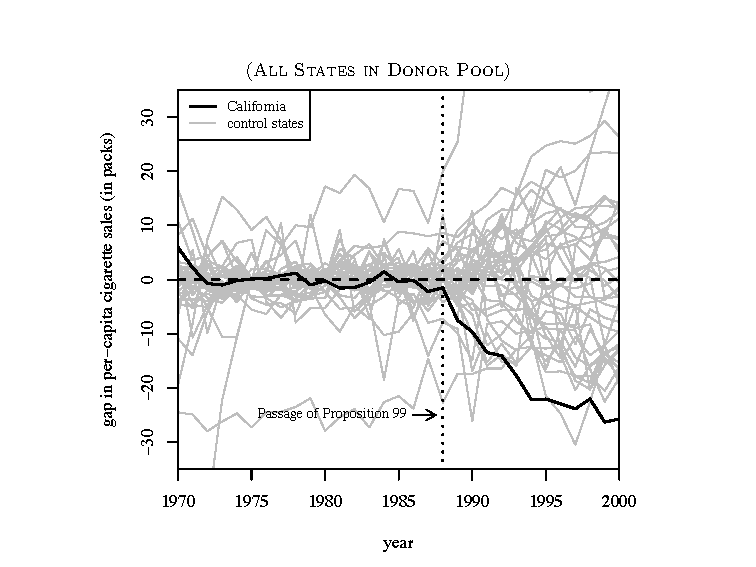
\includegraphics[scale=0.75]{./lecture_includes/abadie_7.pdf}
	\end{figure}
\end{frame}

\begin{frame}{Smoking Gap for CA and 34 control states}
	
	\begin{figure}
	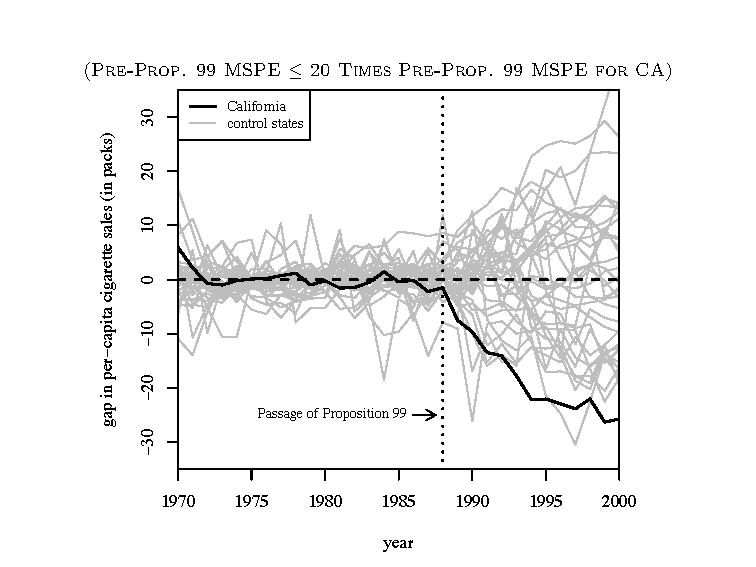
\includegraphics[scale=0.75]{./lecture_includes/abadie_8.pdf}
	\end{figure}
\end{frame}

\begin{frame}{Smoking Gap for CA and 29 control states}
	
	\begin{figure}
	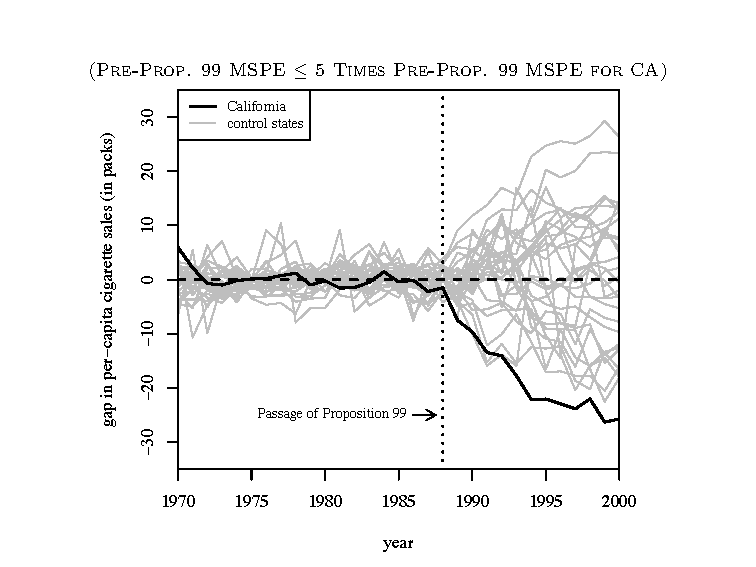
\includegraphics[scale=0.75]{./lecture_includes/abadie_9.pdf}
	\end{figure}
\end{frame}

\begin{frame}{Smoking Gap for CA and 19 control states}
	
	\begin{figure}
	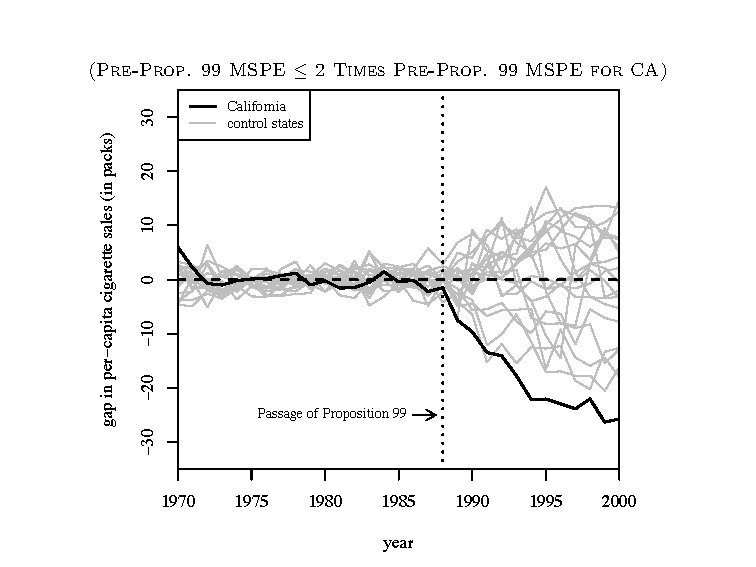
\includegraphics[scale=0.75]{./lecture_includes/abadie_10.pdf}
	\end{figure}
\end{frame}

\begin{frame}{Ratio Post-Prop. 99 RMSPE to Pre-Prop. 99 RMSPE}

	\begin{figure}
	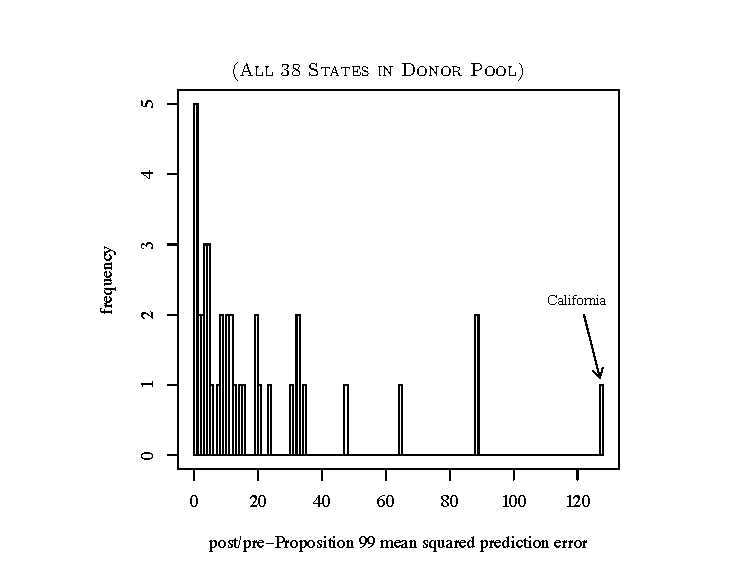
\includegraphics[scale=0.75]{./lecture_includes/abadie_11.pdf}
	\end{figure}
\end{frame}




\begin{frame}{Coding exercise}
	
	\begin{itemize}
	\item The US has the highest prison population of any OECD country in the world 
	\item 2.1 million are currently incarcerated in US federal and state prisons and county jails
	\item Another 4.75 million are on parole
	\item From the early 1970s to the present, incarceration and prison admission rates quintupled in size
	\end{itemize}
\end{frame}



\begin{frame}[plain]

\begin{figure}
\includegraphics[scale=0.5]{./lecture_includes/cook2010.pdf}
\end{figure}
\end{frame}


\begin{frame}{Prison constraints}

	
	\begin{itemize}
	\item Prisons are and have been at capacity for a long time so growth in imprisonment would bite on state corrections
	\item Managing increased flows can only be solved by the following:
		\begin{itemize}
		\item Prison construction
		\item Overcrowding
		\item Paroles
		\end{itemize}
	\item Texas chooses overcrowding
	\end{itemize}
\end{frame}



\begin{frame}{Ruiz v. Estelle 1980}

	
	\begin{itemize}
		\item Class action lawsuit against TX Dept of Corrections (Estelle, warden). 
		\item TDC lost.  Lengthy period of appeals and legal decrees.  
		\item Lengthy period of time relying on paroles to manage flows
	\end{itemize}
\end{frame}

\begin{frame}[shrink=30,plain]
\begin{figure}

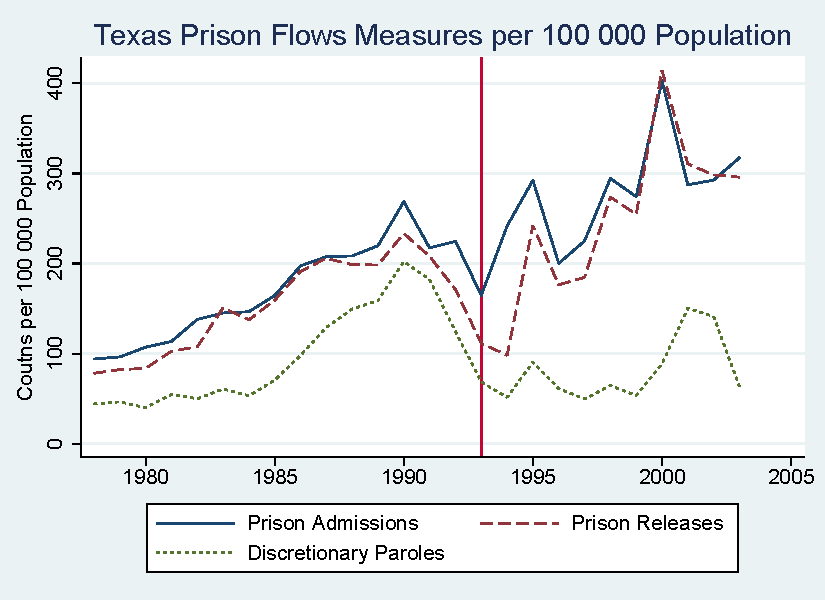
\includegraphics{./lecture_includes/flow_rate_figure.pdf}
\end{figure}
\end{frame}


\begin{frame}{Texas prison boom}

Governor Ann Richards (D) 1991-1995
		\begin{itemize}
		\item Operation prison capacity increased 30-35\% in 1993, 1994 and 1995. 
		\item Prison capacity increased from 55,000 in 1992 to 130,000 in 1995.  
		\item Building of new prisons (private and public)
		\end{itemize} 
\end{frame}


\begin{frame}[shrink=30,plain]

\begin{figure}
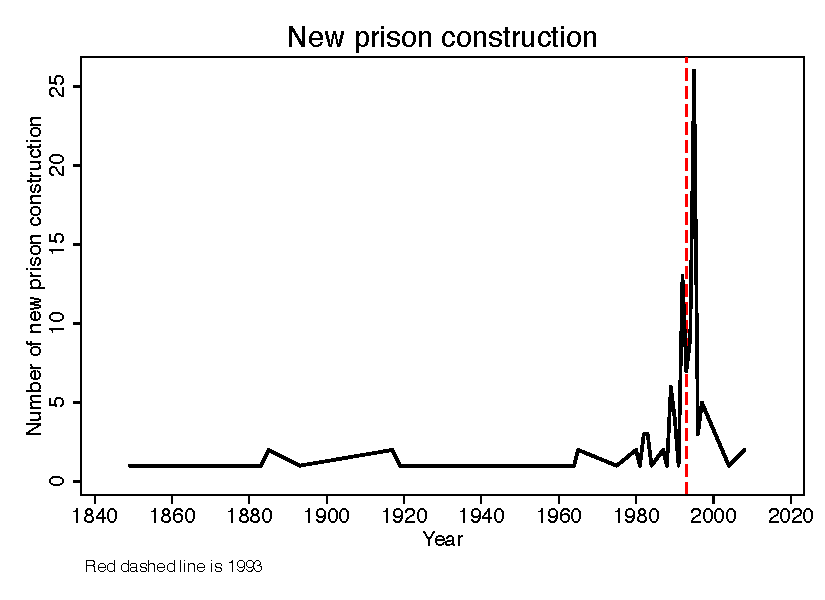
\includegraphics{./lecture_includes/tdcj.pdf}
\end{figure}
\end{frame}


\begin{frame}[shrink=30,plain]
\begin{figure}
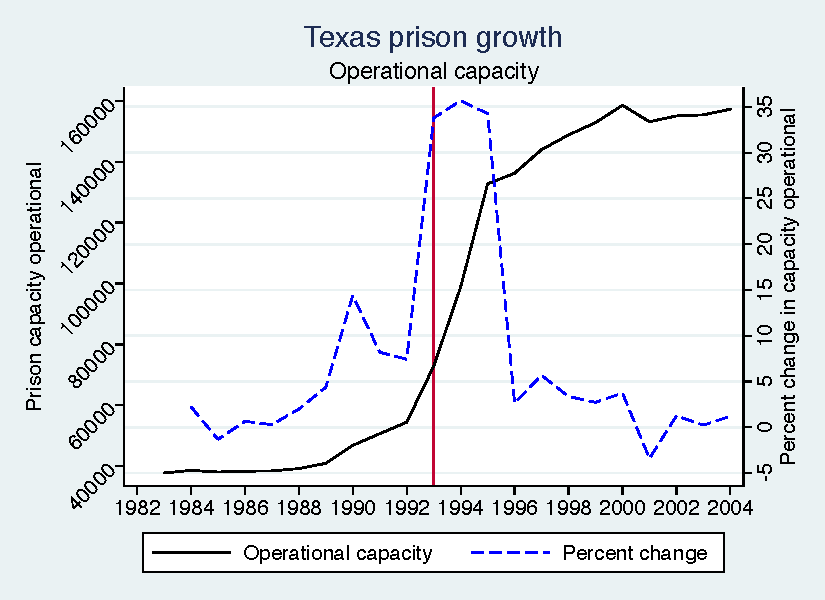
\includegraphics{./lecture_includes/capacity_operational_texas.pdf}
\end{figure}
\end{frame}



\begin{frame}[shrink=30,plain]

\begin{figure}
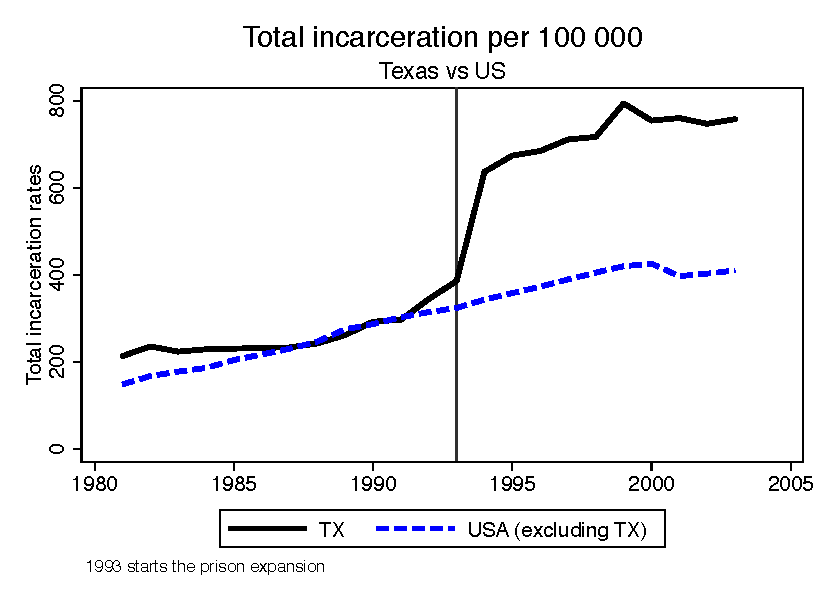
\includegraphics{./lecture_includes/total_incarceration.pdf}
\end{figure}
\end{frame}

\begin{frame}[shrink=30,plain]

\begin{figure}
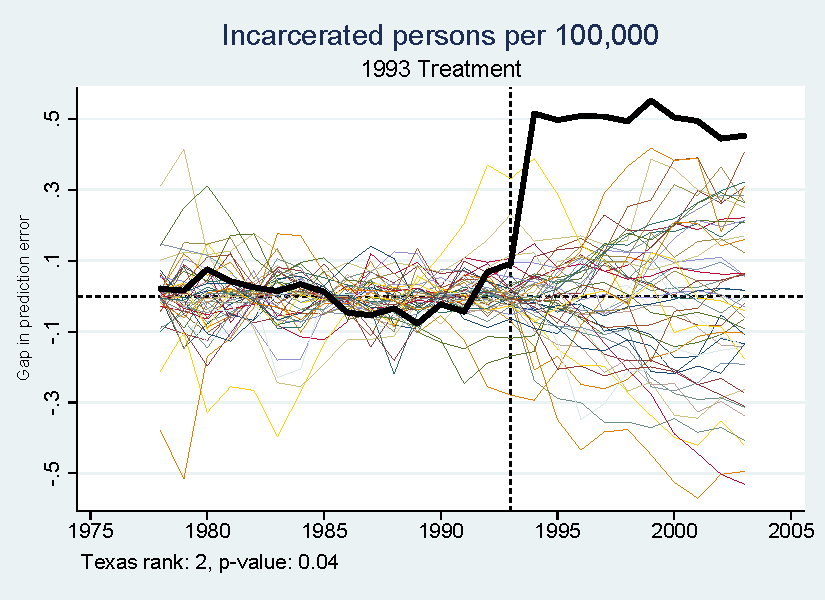
\includegraphics{./lecture_includes/synth_placebo_totalincarceration1993.pdf}
\end{figure}
\end{frame}





\begin{frame}{Coding together}

\begin{itemize}
\item Let's go to Mixtape Sessions repository now into /Labs/Texas 
\item I'll walk us through the Stata and R code so you understand the syntax and underlying logic
\item But then I have us a practice assignment 
\end{itemize}

\end{frame}



\subsection{Augmented Synthetic Control}

\begin{frame}{Introducing Augmented Synthetic Control}
\begin{itemize}
\item Synthetic control has built in constraints forcing weights to be non-negative
\item Convex hull constraint ensures that synth is a feasible counterfactual in that it is formed by a combination of control units similar on pre-intervention characteristics
\item Improves the validity of the estimated effect as there exists interpolated comparison group; similar to common support concept
\item But, the convex hull constraint reduces extrapolation bias from comparing dissimilar units, but at the cost of failing to find matches at all
\end{itemize}

\end{frame}


\begin{frame}

\begin{quote}
``The applicability of the [ADH2010] method requires a sizable number of pre-intervention periods. The reason is that the credibility of a synthetic control depends upon how well it tracks the treated unit’s characteristics and outcomes over an extended period of time prior to the treatment. \textbf{We do not recommend using this method when the pretreatment fit is poor or the number of pretreatment periods is small}. A sizable number of post-intervention periods may also be required in cases when the effect of the intervention emerges gradually after the intervention or changes over time.'' (my emphasis, Abadie, et al. 2015)
\end{quote}

\end{frame}

\begin{frame}{What is augmented synthetic control?}

\begin{itemize}
\item Eli Ben-Michael, Avi Feller and Jesse Rothstein present a modification to ADH in which they allow for negative weights, but only minimally so
\item This model will ``augment'' the original synthetic control model by adjusting for pre-treatment imbalance using doubly robust bias adjustment 
\item Augmentation is conservative; it uses \textbf{penalized ridge regression} but with constraints such that the negative weighting is only to the convex hull, not to the center of the convex hull
\end{itemize}

\end{frame}




\begin{frame}{Gist of their argument}

\begin{enumerate}
\item ADH (``synth'') needs perfect fit and so is biased in practical settings due to the curse of dimensionality as it won't be the case we get weights constrained to be ``on the simplex''
\item Their augmentation will introduce an outcome model to estimate the bias caused by covariate imbalance 
\item Introduces ridge regularization linear regression to estimate new weights to reweight synth
\item Think of it as ``bias reduction'' like Abadie and Imbens (2011) plus it will have doubly robust properties and be equivalent to inverse probability weighting
\item When synth is imbalanced, augmented synth will reduce bias reweighting and bias correction, and when synth is balanced, they are the same
\end{enumerate}

\end{frame}


\begin{frame}{Gist of their argument}

\begin{enumerate}
\item Ridge regularization linear regression used to estimate weights used to reweight the original synth model
\item If synth is imbalanced, augmented synth reducees bias by reweighting and bias correction
\item When synth is balanced, the augmented and original synth are identical (but in practice, they won't be identical)
\item They argue synth DiD can be seen as a special case of augmented synth
\end{enumerate}

\end{frame}


\begin{frame}{Some topical observations}

\begin{itemize}
\item Foregoes estimating \emph{donor pool unit weights} (e.g., ADH, synth did, MCNN)
\item Synth sequels are using penalization/regularization for estimation
\item Relaxes some of the original ADH constraints, like non-negative weights (i.e., no extrapolation)
	\begin{itemize}
	\item This is used to address bias caused by imbalance
	\item Negative weights puts them back in the convex hull which recall we need
	\item They argue synth DiD can be seen as a special case of augmented synth
	\end{itemize}
\end{itemize}

\end{frame}



\begin{frame}{Notation}

\begin{itemize}
\item Observe $J+1$ units over $T$ time periods
\item Unit $1$ will be treated at time period $T_0=T-1$ (we allow for unit $1$ to be an average over treated units)
\item Units $j=2 $ to $J+1$ (using ADH original notation) are ``never treated''
\item $D_j$ is the treatment indicator
\end{itemize}

\end{frame}


\begin{frame}[plain,shrink=20]
\begin{center}
\textbf{Pre-treatment outcomes}
\end{center}

\begin{center}
\[ \left( \begin{array}{ccccc}
    Y_{11} & Y_{12} & Y_{13} & \dots  & Y_{1T}^1 \\
    Y_{21} & Y_{22} & Y_{23} & \dots  & Y_{2T}^0  \\
    \vdots & \vdots & \vdots & \ddots & \vdots \\
    Y_{N1} & Y_{i2} & Y_{i3} & \dots  & Y_{NT}^0
\end{array} \right) \equiv
\left( \begin{array}{ccccc}
    X_{11} & X_{12} & X_{13} & \dots  & Y_{1} \\
    X_{21} & X_{22} & X_{23} & \dots  & Y_{2}  \\
    \vdots & \vdots & \vdots & \ddots & \vdots \\
    X_{N1} & X_{i2} & X_{i3} & \dots  & Y_{N}
\end{array} \right) \equiv
\left( \begin{array}{cc}
    X_{1} & Y_{1} \\
    X_{0} & Y_{0}  \\
\end{array} \right)
\]

\end{center}

This is a model of 2x2 (i.e., single last period block structure, not staggered roll out)

\bigskip

The last column is always post-treatment and switches from $Y^1$ to $Y$. 

\bigskip

The last column is just showing a top row of the treated unit 1 and the bottom row of all the donor pool (i.e., we will use $X_0$ and $Y_0$ to represent all the donor pool units)

\end{frame}


\begin{frame}{Optimal weights}

Synth minimizes the following norm:

\begin{eqnarray*}
\textrm{min}_w = || V_X^{1/2} (X_1 - X_0'w) ||_2^2 + \psi \sum_{D_j=0}f(w_j)\\
\textrm{s.t. }\sum_{j=2}^N w_{j} =1 \textrm{ and } w_j \geq 0
\end{eqnarray*}

$Y_0'w*$ (i.e., optimally weighted donor pool) is the unit 1 ``synthetic control'' 

\end{frame}


\begin{frame}{Predicting counterfactuals}

Synth minimizes the following norm:

\begin{eqnarray*}
\textrm{min}_w = || V_X^{1/2} (X_1 - X_0'w) ||_2^2 + \psi \sum_{D_j=0}f(w_j)\\
\textrm{s.t. }\sum_{j=2}^N w_{j} =1 \textrm{ and } w_j \geq 0
\end{eqnarray*}

We are hoping that $\widehat{Y}_1^0$ with $Y_0' {w}^{*}$ based on ``perfect fit'' pre-treatment

\end{frame}




\begin{frame}{$V_X$ matrix}

Synth minimizes the following norm:

\begin{eqnarray*}
\textrm{min}_w = || V_X^{1/2} (X_1 - X_0'w) ||_2^2 + \psi \sum_{D_j=0}f(w_j)\\
\textrm{s.t. }\sum_{j=2}^N w_{j} =1 \textrm{ and } w_j \geq 0
\end{eqnarray*}

$V_x$ is the ``importance'' matrix on $X_0$ (Stata default chooses $V_x$ that min pre-treatment MSE).
\end{frame}

\begin{frame}{Penalizing the weights with ridge}

Synth minimizes the following norm:

\begin{eqnarray*}
\textrm{min}_w = || V_X^{1/2} (X_1 - X_0'w) ||_2^2 + \psi \sum_{D_j=0}f(w_j)\\
\textrm{s.t. }\sum_{j=2}^N w_{j} =1 \textrm{ and } w_j \geq 0
\end{eqnarray*}

Modification to the original synthetic control model is the inclusion of the penalty term. ``The choice of penalty is less central when weights are constrained to be on the simplex, but becomes more important when we relax this constrain.''

\end{frame}

\begin{frame}{Convex hull}

Synth minimizes the following norm:

\begin{eqnarray*}
\textrm{min}_w = || V_X^{1/2} (X_1 - X_0'w) ||_2^2 + \psi \sum_{D_j=0}f(w_j)\\
\textrm{s.t. }\sum_{j=2}^N w_{j} =1 \textrm{ and } w_j \geq 0
\end{eqnarray*}

These weights will be used to address imbalance, not so much the control units, bc this method is for when the weighted controls are still outside the convex hull (``simplex'')

\end{frame}



\begin{frame}{Slight change in synth notation}

\begin{itemize}
\item Assume that our outcome, $Y_{jt}$, follows a factor model where $m(.)$ are pre-treatment outcomes: $$ Y_{jt}^0 = m_{jt} + \varepsilon_{jt}$$
\item Since $\widehat{m(.)}$ estimates the post-treatment outcome, let's view it as estimated bias, analogous to bias correction for inexact matching (Abadie and Imbens 2011)
\end{itemize}

\end{frame}



\begin{frame}{Bias correction}

 $$ Y_{jt}^0 = m_{jt} + \varepsilon_{jt}$$

\begin{itemize}
\item When the weights achieve exact balance, the bias of synthetic control decreases with $T$
\item The intuition is that for a large $T$ ($T$ not transitory shocks), you achieve balance by balancing the latent parameter on the unobserved heterogeneity in our factor model
\end{itemize}

\end{frame}



\begin{frame}{Common practice}

\begin{itemize}
\item Usually the number of time periods isn't much larger than the number of units
\item And exact balance rarely holds, which if it doesn't hold, then the unobserved heterogeneity also doesn't get deleted
\end{itemize}

\end{frame}


\begin{frame}{Treatment and control units}

	\begin{figure}
	\includegraphics[scale=0.07]{./lecture_includes/convexhull_1.png}
	\end{figure}

\end{frame}

\begin{frame}{Convex hull -- ideal for synth}

	\begin{figure}
	\includegraphics[scale=0.07]{./lecture_includes/convexhull_2.png}
	\end{figure}

\end{frame}

\begin{frame}{Outside the convex hull bc of dimensionality}

	\begin{figure}
	\includegraphics[scale=0.07]{./lecture_includes/convexhull_3.png}
	\end{figure}

\end{frame}

\begin{frame}{Outside the convex hull bc of dimensionality}

	\begin{figure}
	\includegraphics[scale=0.07]{./lecture_includes/convexhull_4.png}
	\end{figure}

\end{frame}


\begin{frame}{Estimating the bias}

\begin{itemize}
\item Adjust the synthetic control approach to adjust for poor fit pre-treatment.
\item Recall our factor model -- let $\widehat{m}_{jT}$ be an estimator for the post-treatment control potential outcome $Y_{jT}^0$.
\item The augmented synthetic control estimator for $Y_{jt}^0$ is on the next slide
\end{itemize}


\end{frame}




\begin{frame}{Setup of the estimator}

Let's adjust synthetic control for this bias.  First we'll apply the \textbf{bias correction}.  Then we'll do the doubly robust augmented \textbf{inverse probability weighting}. Let $Y_1^{aug,0}$ be the augmented potential outcome

\begin{eqnarray*}
Y_1^{aug,0} &=& \sum_{D_j=0} \widehat{w}_j^{synth} Y_{j} + \widehat{m}(X_1) - \sum_{D_j=0} \widehat{w}_j \widehat{m}(X_j) \\
&=& \widehat{m}(X_1) + \sum_{D_j=0} \widehat{w_j}(Y_j - \widehat{m}(X_j))
\end{eqnarray*}

\end{frame}


\begin{frame}{Interpreting line 1}

\begin{eqnarray*}
Y_1^{aug,0} &=& \sum_{D_j=0} \widehat{w}_j^{synth} Y_{jT} + \bigg (\widehat{m}_{1T} - \sum_{D_j=0} \widehat{w}_j^{synth}\widehat{m}_{jT} \bigg ) \\
&=& \widehat{m}_{1T} + \sum_{D_j=0} \widehat{w}_j^{synth} (Y_{jT} - \widehat{m}_{jT})
\end{eqnarray*}

(1) Note how in the first line the traditional synthetic control weighted outcomes are corrected by the imbalance in a particular function of the pre-treatment outcomes $\widehat{m}$. 
\end{frame}




\begin{frame}{Interpreting line 1}

\begin{eqnarray*}
Y_1^{aug,0}  &=& \sum_{D_j=0} \widehat{w}_j^{synth} Y_{jT} + \bigg (\widehat{m}_{1T} - \sum_{D_j=0} \widehat{w}_j^{synth}\widehat{m}_{jT} \bigg ) \\
&=& \widehat{m}_{1T} + \sum_{D_j=0} \widehat{w}_j^{synth} (Y_{jT} - \widehat{m}_{jT})
\end{eqnarray*}

(1) Since $\widehat{m}$ estimates the post-treatment outcome, we can view this as an estimate of the bias due to imbalance, which is similar to how you address imbalance in matching with a bias correction formula (Abadie and Imbens 2011). 

\end{frame}





\begin{frame}{Interpreting line 1}

\begin{eqnarray*}
Y_1^{aug,0}  &=& \sum_{D_j=0} \widehat{w}_j^{synth} Y_{jT} + \bigg (\widehat{m}_{1T} - \sum_{D_j=0} \widehat{w}_j^{synth}\widehat{m}_{jT} \bigg ) \\
&=& \widehat{m}_{1T} + \sum_{D_j=0} \widehat{w}_j^{synth} (Y_{jT} - \widehat{m}_{jT})
\end{eqnarray*}

(1) I actually cover the bias correction of Abadie and Imbens 2011 in the mixtape!  The subclassification chapter

\end{frame}


\begin{frame}{Interpreting line 1}
\begin{eqnarray*}
Y_1^{aug,0}  &=& \sum_{D_j=0} \widehat{w}_j^{synth} Y_{jT} + \bigg (\widehat{m}_{1T} - \sum_{D_j=0} \widehat{w}_j^{synth}\widehat{m}_{jT} \bigg ) \\
&=& \widehat{m}_{1T} + \sum_{D_j=0} \widehat{w}_j^{synth} (Y_{jT} - \widehat{m}_{jT})
\end{eqnarray*}

(1) So if the bias is small, then synthetic control and augmented synthetic control will be similar because that interior term will be zero.

\end{frame}

\begin{frame}{Interpreting line 2}

\begin{eqnarray*}
Y_1^{aug,0}  &=& \sum_{D_j=0} \widehat{w}_j^{synth} Y_{jT} + \bigg (\widehat{m}_{1T} - \sum_{D_j=0} \widehat{w}_j^{synth}\widehat{m}_{jT} \bigg ) \\
&=& \widehat{m}_{1T} + \sum_{D_j=0} \widehat{w}_j^{synth} (Y_{jT} - \widehat{m}_{jT})
\end{eqnarray*}

(2) The second equation is equivalent to a double robust estimation which begins with an outcome model but then re-weights it to balance residuals.


\end{frame}



\begin{frame}{Interpreting line 2}

\begin{eqnarray*}
Y_1^{aug,0}  &=& \sum_{D_j=0} \widehat{w}_j^{synth} Y_{jT} + \bigg (\widehat{m}_{1T} - \sum_{D_j=0} \widehat{w}_j^{synth}\widehat{m}_{jT} \bigg ) \\
&=& \widehat{m}_{1T} + \sum_{D_j=0} \widehat{w}_j^{synth} (Y_{jT} - \widehat{m}_{jT})
\end{eqnarray*}

(2) The second equation has a connection to inverse probability weighting (they show this in an appendix)


\end{frame}
\begin{frame}{Ridge Augmented SCM}

\begin{eqnarray*}
\textrm{arg min}_{\eta_0,\eta} \frac{1}{2} \sum_{D_j=0} (Y_j - (\eta_0 + X_j'\eta))^2 + \lambda^{ridge} || \eta ||_2^2
\end{eqnarray*}Here we estimate $\widehat{m}(X_j)$ with ridge regularized linear model and penalty hyper parameter $\lambda^{ridge}$. Sorry -- this is not the same $\lambda$. I didn't create this notation though! Once we have those, we adjust for imbalance using the $\widehat{\eta}^{ridge}$ parameter as a weight on the outcome model itself. 

\end{frame}

\begin{frame}{Ridge Augmented SCM}

\begin{eqnarray*}
\textrm{arg min}_{\eta_0,\eta} \frac{1}{2} \sum_{D_j=0} (Y_j - (\eta_0 + X_j'\eta))^2 + \lambda^{ridge} || \eta ||_2^2
\end{eqnarray*}Once we have those, we adjust for imbalance using the $\widehat{\eta}^{ridge}$ parameter as a weight on the outcome model itself. 

\end{frame}




\begin{frame}{Go back to that weighting but use the ridge parameters}

\begin{eqnarray*}
Y_1^{aug,0} &=& \sum_{D_j=0} \widehat{w}_j^{synth} Y_{j} + \bigg ( X_1 - \sum_{D_j=0} \widehat{w}_j^{synth} X_j \bigg ) \widehat{\eta}^{ridge} \\
&=& \sum_{D_j=0} \widehat{w}_j^{aug}Y_j
\end{eqnarray*}What you're trying to do is adjust with the $\widehat{w}_j^{aug}$ weights to improve balance.  

\end{frame}


\begin{frame}{The ridge weights are key to the augmentation}

\begin{eqnarray*}
\widehat{w}_j^{aug} = \widehat{w}_j^{synth} + (X_j - X_0' \widehat{w}_j^{synth}) ' (X_0'X_0 + \lambda I_{T_0})^{-1}X_i
\end{eqnarray*}

The second term is adjusting the original synthetic control weights, $w_j^{synth}$ for better balance. Again remember -- we are trying to address the bias due to imbalance. You can achieve better balance, but at higher variance and can introduce negative weights. 

\end{frame}



\begin{frame}{Ridge will allow negative weights via extrapolation}

\begin{eqnarray*}
\widehat{w}_j^{aug} = \widehat{w}_j^{synth} + (X_j - X_0' \widehat{w}_j^{synth}) ' (X_0'X_0 + \lambda I_{T_0})^{-1}X_i
\end{eqnarray*}

Relaxing the constraint from synth that weights be non-negative, as non-negative weights prohibit extrapolation. But we don't have synthetic control on the simplex, so we \emph{must} extrapolate, otherwise synth will be biased.

\end{frame}



\begin{frame}{Summarizing and some comments}

\begin{itemize}
\item When the treated unit lies in the convex hull of the control units so that the synth weights exactly balance lagged outcomes, then SCM and Ridge ASCM are the same
\item When synth weights do not achieve exact balance, Ridge ASCM will use negative weights to extrapolate from the convex hull to the control units
\item The amount of extrapolation will be determined by how much imbalance we're talking about and the estimated hyperparameter $\widehat{\lambda}^{ridge}$
\item When synth has good pre-treatment fit or when $\lambda^{ridge}$ is large, then adjustment will be small and the augmented weights will be close to the SCM weights
\end{itemize}

\end{frame}



\begin{frame}{Intuition}

Ridge begins at the center of control units, while Ridge ASCM begins at the synth solution. Both move towards an exact fit solution as the hyperparameter is reduced. It is possible to achieve the same level of balance with non-negative weights.  Both ridge and Ridge ASCM extrapolate from the support of the data to improve pre-treatment fit relative to synth alone. Let's look at a picture!


\end{frame}



\begin{frame}[plain]

	\begin{figure}
	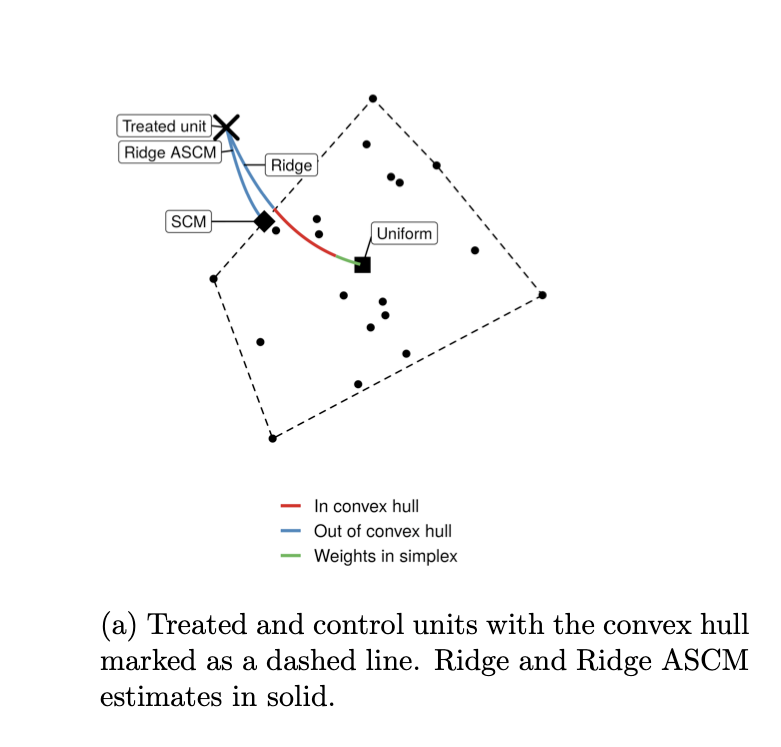
\includegraphics[scale=0.5]{./lecture_includes/aug_1.png}
	\end{figure}
	
\end{frame}	


\begin{frame}{Conformal Inference}

Inference will be based on ``conformal inference'' method by Chernozhukov et al. (2019).  We will get 95\% point-wide confidence intervals. They also outline a jackknife method by Barber et al (2019). 

\end{frame}


\begin{frame}{Steps of conformal Inference}

\begin{enumerate}
\item [1] Choose a sharp null (i.e., no unit-level treatment effects, $\delta_0=0$)
	\begin{itemize}
	\item Enforce the null by creating an adjusted post-treatment outcome for the treated unit equal to $Y_{1T}-\delta_0$ (in other words, we get CI on the post-treatment outcomes, not the pre-treatment)
	\item Augment the original dataset to include the post-treatment time period $T$ with the adjusted outcome and use the estimator to obtain the adjusted weights $\widehat{w(\delta_0)}$
	\item Compute a p-value by assessing whether the adjusted residual conforms with the pre-treatment residuals (see Appendix A for the exact formula)
	\end{itemize}
\end{enumerate}


\end{frame}


\begin{frame}{Steps of conformal Inference}

\begin{enumerate}
\item [2] Compute a level $\alpha$ for $\delta$ by inverting the hypothesis test (see Appendix A for the exact formula)
	\begin{itemize}
	\item Chernozhukov et al. (2019) provide several conditions for which approximate or exact finite-sample validity of the $p$-values (and hence coverage of the predicted confidence intervals) can be achieved)
	\end{itemize}
\end{enumerate}

See Appendix A for more details

\end{frame}


\begin{frame}{Simulations (summarized)}

\begin{itemize}
\item They examine the performance of synth against ridge, Augmented synth with ridge regularization, demeaned synth, and fixed effects under four DGP
\item Augmenting synth with a ridge outcome regression reduces bias relative to synth alone in all four simulations
\item This underscores the importance of the recommendation Abadie, et al. (2015) make which is that synth should be used in settings with excellent pre-treatment fit
\item They also examine a real situation involving Kansas tax cuts in 2012
\end{itemize}

\end{frame}

\imageframe{./lecture_includes/aug_5.png}

\imageframe{./lecture_includes/aug_6.png}

\begin{frame}{Couple of minor points}

\begin{itemize}
\item Hyper parameter chosen using cross validation
\item This can be extended to auxiliary covariates as opposed to just lagged outcomes (section 6)
\end{itemize}

\end{frame}



\begin{frame}{Some minor points}

\begin{itemize}
\item We've motivated augmented synth as a kind of bias correction, but you can also think of it as correcting synth with an inverse probability weight (Appendix E)
\item There's an implicit estimate of a propensity score model with ridge regularization
\item Weights are odds of treatment (they're ATT weights), i.e., they're the inverse probability weighting scheme from Abadie (2005)
\end{itemize}

\end{frame}


\begin{frame}{Augmented synth is better}

\begin{itemize}
\item In conclusion, synthetic control is best when pre-treatment fit is excellent, otherwise it is biased
\item Synthetic control avoids extrapolation by restricting weights to be non-negative and sum to one
\item Ridge regression augmentation will allow for a degree of extrapolation to achieve pre-treatment balance and that creates negative weights
\item Augmented synth will dominate synth in those instances by extrapolating outside the convex hull
\item They also say synth DiD is a special case of their augmented synth method, which is interesting as synth DiD is also meant to nest all such modifications too (but they don't discuss augmented synth)
\end{itemize}

\end{frame}



\begin{frame}{R code}

R: \url{https://github.com/ebenmichael/augsynth}

\end{frame}

\section{Concluding remarks}

\begin{frame}{Summarizing}

\begin{itemize}
\item People call the RCT the ``gold standard'' -- why?  
\item Because randomization causes $[Y^1]$ and $E[Y^0]$ to be distributed equally in treatment and control forcing selection bias to be zero in large samples
\item Very hard to imagine a situation where randomization would make things worse

\end{itemize}

\end{frame}

\begin{frame}{Summarizing}

\begin{itemize}
\item Randomized treatments are great but not always available 
\item Can't randomize parental methamphetamine abuse (my paper) to see its causal effect, if any, on child abuse but obviously important question
\item Theoretically, randomization is not necessary -- parallel trends can also be used to estimate the ATT (just not the ATE)

\end{itemize}

\end{frame}

\begin{frame}{Summarizing}

\begin{itemize}
\item Difference-in-differences is a straightforward design -- four averages and three differences
\item Can be estimated with OLS, but with differential timing, be sure to match on units not treated
\item But sometimes parallel trends is too strong an assumption
\item Synthetic control can be used in its place but it also has a strong assumption and hungry data needs -- the factor model

\end{itemize}

\end{frame}

\begin{frame}{Summarizing}

\begin{itemize}
\item You need long pre-treatment to evaluate the credibility that the treated unit sits in the convex hull
\item Original model uses non-negative weighting to form synthetic control but sometimes that is not possible
\item An alternative is to allow the most conservative negative weighting possible with augmented synth
\item Includes bias correction too and performs better than original but at the expense of extrapolation 

\end{itemize}

\end{frame}

\begin{frame}{Summarizing}

\begin{itemize}
\item Don't use econometrics as a substitute for common sense
\item Be skeptical, always try to find holes in your project, be honest
\item Don't be defensive
\item Shoeleather
\item Good luck

\end{itemize}

\end{frame}






\end{document}
